\documentclass[varwidth=false, border=2pt]{standalone}

\usepackage{pgfplots}
\usepackage{tikz}
\usepackage{nicefrac}
\pgfplotsset{every axis legend/.append style={
at={(0,0)},
anchor=north east}}

\begin{document}
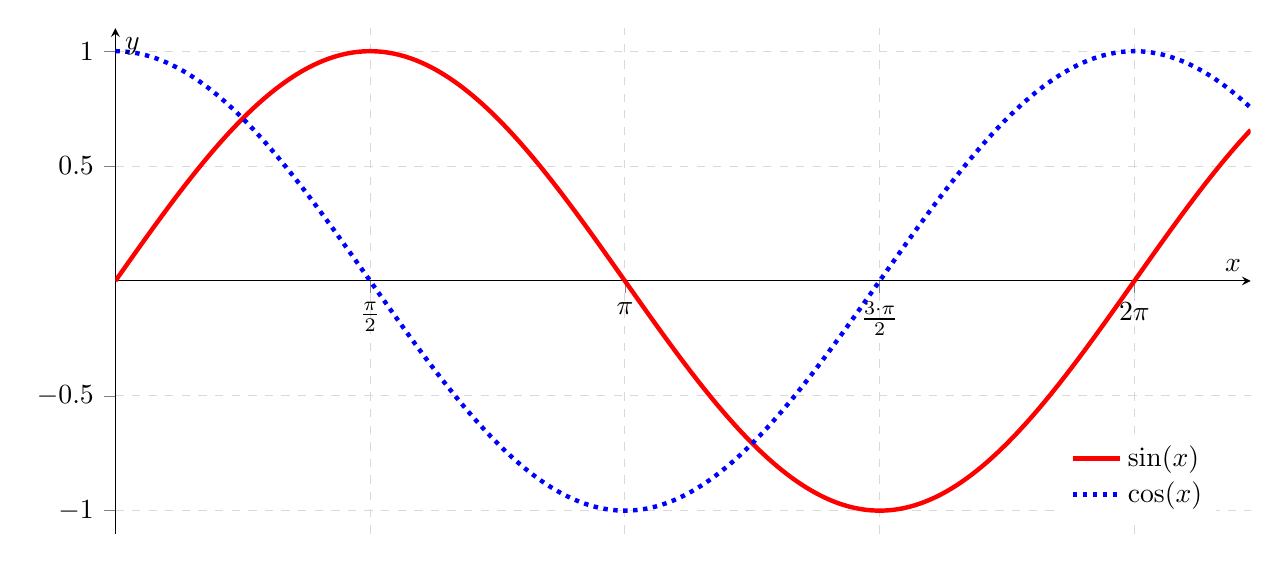
\begin{tikzpicture}
    \begin{axis}[
        axis x line=middle,
        axis y line=middle,
        grid = major,
        width=16cm,
        height=8cm,
        grid style={dashed, gray!30},
        xmin= 0,   % start the diagram at this x-coordinate
        xmax= 7,   % end   the diagram at this x-coordinate
        ymin=-1.1,   % start the diagram at this y-coordinate
        ymax= 1.1,   % end   the diagram at this y-coordinate
        xlabel=$x$,
        ylabel=$y$,
        xtick={0,pi/2,pi,1.5*pi,2*pi},
        xticklabels={0,$\frac{\pi}{2}$,$\pi$,$\frac{3 \cdot \pi}{2}$,$2 \pi$},
        legend cell align=left,
        legend pos=south east,
        legend style={draw=none},
        tick align=outside,
        enlargelimits=false]
      % plot the function
      \addplot[domain=0:7, red, ultra thick,samples=1000] {sin(deg(x))};
      \addplot[domain=0:7, blue, ultra thick,dotted,samples=1000] {cos(deg(x))};
      \legend{$\sin(x)$, $\cos(x)$}
    \end{axis}
\end{tikzpicture}
\end{document}
